\documentclass[a4paper]{jpconf}
\usepackage{graphicx,amsmath}
\bibliographystyle{iopart-num}

\begin{document}
\title{Upgrades to the SINQ Cold Neutron Source}

\author{R M Bergmann, U Filges, D Kiselev, T Reiss, V Talanov and M Wohlmuther}

\address{Paul Scherrer Institut, 5232 Villigen, Switzerland}

\ead{ryan.bergmann@psi.ch}

\begin{abstract}Changing the configuration of the cold neutron source during an extended shutdown of Swiss Spallation Neutron Source (SINQ) is being considered for improving performance of the instruments that use the cold source.  The cold neutron source consists of a 20 L volume of liquid D$_2$ at approximately 25 K.  Previous upgrades included adding a re-entrant hole into one side of the D$_2$ volume to allow cold neutrons to stream uninhibited from the center of the source towards the instrument neutron guides.  Calculations done prior to these changes predicted cold neutron fluence gains from 1.2 to 1.6, with gains increasing with wavelength. These increases have not been observed, and it is suspected that the re-entrant hole is not fully voided.  Voiding the re-entrant hole relies on radiative heating to boil D$_2$ which in turn fills the re-entrant hole cavity, pushing the liquid D$_2$ out.  Proposed plans include making the re-entrant hole external (ensuring that it is not filled with liquid D$_2$), redesigning the re-entrant hole geometry to be more optically ideal, introducing a Pb-208 reflector to minimize cold neutron up-scattering from the surrounding D$_2$O moderator tank, and implementing a small liquid H$_2$ volume to provide a cold neutron “hot spot” for certain instruments.  These changes are predicted to increase neutron fluence between 1.1 to 2.0 times the current levels, depending on instrument location, view, and wavelengths of interest.
\end{abstract}

\ack{This work was supported by Swiss National Science Foundation grant 200021\_150048/1.}

\section{Introduction}

There is a planned shutdown of the Swiss Spallation Neutron Source (SINQ) in 2017, which provides an opportunity for changes to be made to the liquid deuterium cold neutron source \cite{rueegg_icans}.  The 20 liter volume of liquid D$_2$ at approximately 25 K is located within the D$_2$O moderator tank surrounding the lead spallation target.  The innermost face of the cold source is approximately 35 cm away from the center of the target.  In the planned upgrade strategies, no changes to the surrounding aluminum and zirconium safety hulls will be made, and no changes to the insert tube structure will be made.  I.e., all changes must fit into the existing multi-walled insert geometry.  

\section{Re-entrant Hole}

The goal of the re-entrant hole (REH) is to remove scattering and absorbing material between the cold neutron maximum and the direction of interest.  In this case, the cold neutron maximum is at the center of the cold source and the direction of interest is towards the SINQ guide hall.  

The REH is presently a five-sided box with the open face at the bottom.  It sits inside the D$_2$ volume directly next to the wall facing the guide hall.  Voiding this kind of re-entrant hole relies on radiative heating to boil D$_2$ which in turn fills the re-entrant hole cavity with vapor, pushing the liquid D$_2$ out.  Proposed plans include making the re-entrant hole external, ensuring that it is not filled with liquid D$_2$.

Calculations done prior to these changes predicted cold neutron fluence gains from 1.2 to 1.9, with gains increasing with wavelength \cite{atch_icans}. These increases have not been observed, and it is suspected that the re-entrant hole is not fully voided \cite{voided}.  All future designs will have an external REH, which will decouple the fill level from radiation heating and ensure that the REH is never filled with liquid D$_2$.

\section{Simulation Geometry}

Figure \ref{geom} shows a zoomed-in view of the important parts of the MCNP model geometry.  A CAD model of the neutron guide bundles was converted to MCNP geometry by the MCAM and integrated into the model \cite{mcam}.  The target is made of lead rods with zircaloy cladding and is cooled by D$_2$O, the moderator tank is filled with D$_2$O, the cold source is liquid D$_2$, the nozzles with a low-pressure helium mixture, and the shielding and neutron guide structure is steel.  All structural material in the moderator tank is AlMg3, which is shown in yellow in Figure \ref{geom}.

\begin{figure}
\begin{center}
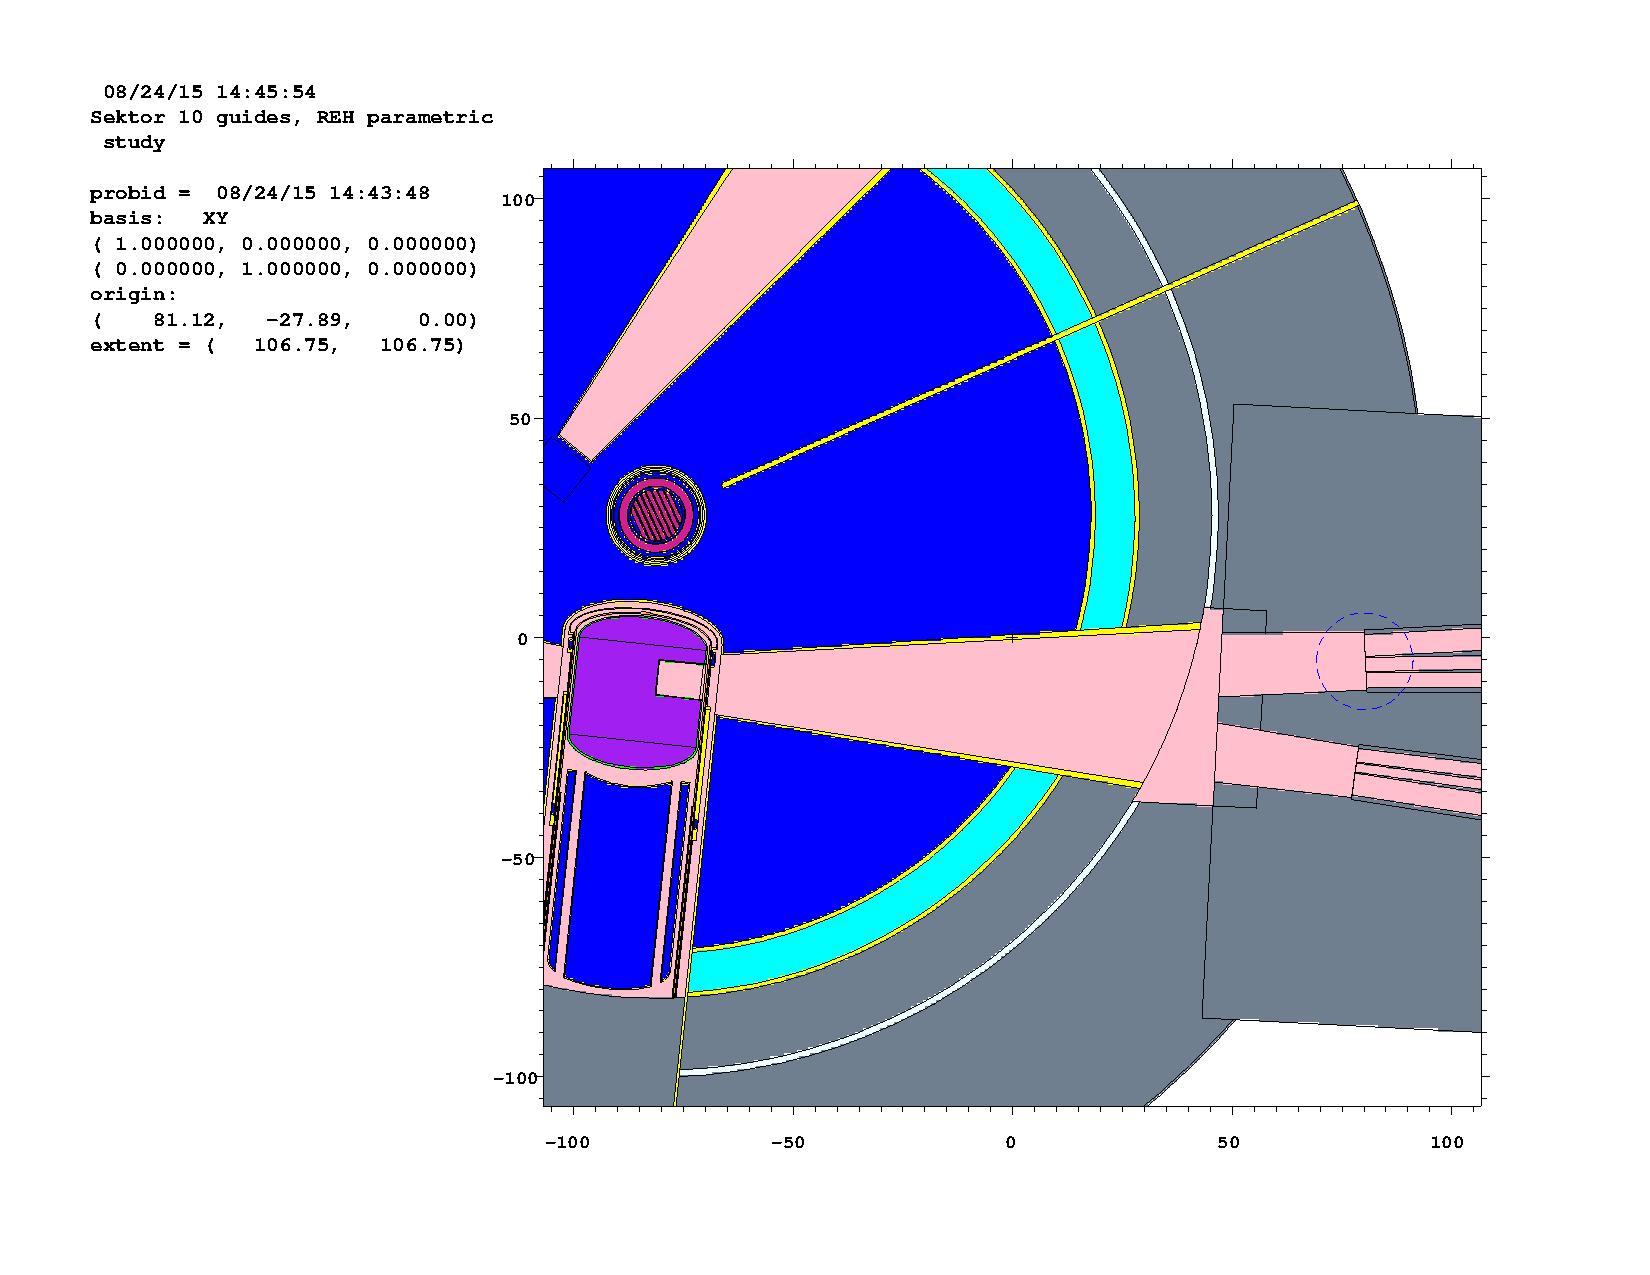
\includegraphics[trim={9.2cm 8cm 4cm 8cm},clip]{graphics/geom.pdf}
\end{center}
\caption{\label{geom}A horizontal slice through the MCNP simulation geometry showing the target (magenta), moderator tank (blue), cold source (purple), nozzle (pink), and neutron guide entrance (grey with circle).}
\end{figure}

\section{Variance Reduction}

Two variance reduction methods were used in conjunction to perform the simulations in a reasonable amount of time.  First, mesh-based weight windows were generated based on the response of a point detector located inside the AMOR neutron guide, 75 cm from the entrance.  The position gives the detector approximately a two degree view towards to cold source.  The generated weight windows serve to increase the number of neutrons in regions that make large contributions to the point detector, which in this case is the cold source. In order to not bias simulation, the weight windwos cause neutrons entering the cold source are split into many neutrons with a lower statistical weight.  

The second variance reduction method used is a ``DXTRAN'' sphere.  This tool is a non-physical sphere that is placed around the guide entrance that causes neutrons to be generated on its surface.  Whenever a neutron undergoes a scattering reaction, the probability of scattering into the sphere's direction is calculated, a line is traced from the scattering location to the sphere's surface, and a neutron is generated at the surface with a weight reduced by the scattering probability and attenuation of the medium in-between.  The generated neutrons are then transported normally inside the sphere \cite{mcnp5,mcnp6}.  This method serves to preferentially scatter neutrons into the direction of the neutron guide instead of relying on probability to scatter them there.

\section{Neutron Guide Response} 

In conjunction with the variance reduction methods described in the previous section, an approximation to how the neutron geuides transport neutrons was also used.  A patch was developed at ORNL and PSI that implements the McStas guide reflectivity model in MCNPX 2.5.0 and 2.7.0 \cite{mcnp_reflectivity, EK_reflectivity}, but the model is analog and is not fully compatible with DXTRAN spheres.  If a neutron is sampled to \emph{not} reflect on a guide surface, it is transmitted into the next cell.  This means that neutron paths have to be sampled multiple times to account for any reflectivity losses, which slows the simulation down.  

Some stability issues were also encountered while using the reflectivity patch in the same simulation as a DXTRAN sphere.  In order to ensure stable runs, the simulation was split into two parts.  First, a simulation was done where a surface source was written at the guide entrance surface.  Any neutrons entering the guide were recorded and terminated.  This source was then used in a second simulation with the guide reflectivity activiated.  This step transported the entering neutrons to the end of the guide where a tally was scored.  Again, this process slowed the simulation down since two MCNP simulations needed to be made for each case.  A guide response approximation was used to eliminate the second run, which simply served to transport the neutrons to the end of the guide.


\subsection{Guide Reflectivity}

The guide reflectivity model implemented in MCNP is identical to that used in McStas \cite{mcnp_reflectivity}.  The reflectivity curve for the current guide in the SINQ hall is shown in Figure \ref{SINQ_reflectivity} and the reflectivity equation and parameter values shown in Eq. \ref{eq:ref} \cite{mcstas}.  The values shown are the same for all the guides in the SINQ hall \cite{SINQ_guide_values}.

\begin{figure}[h]
\begin{minipage}{14pc}
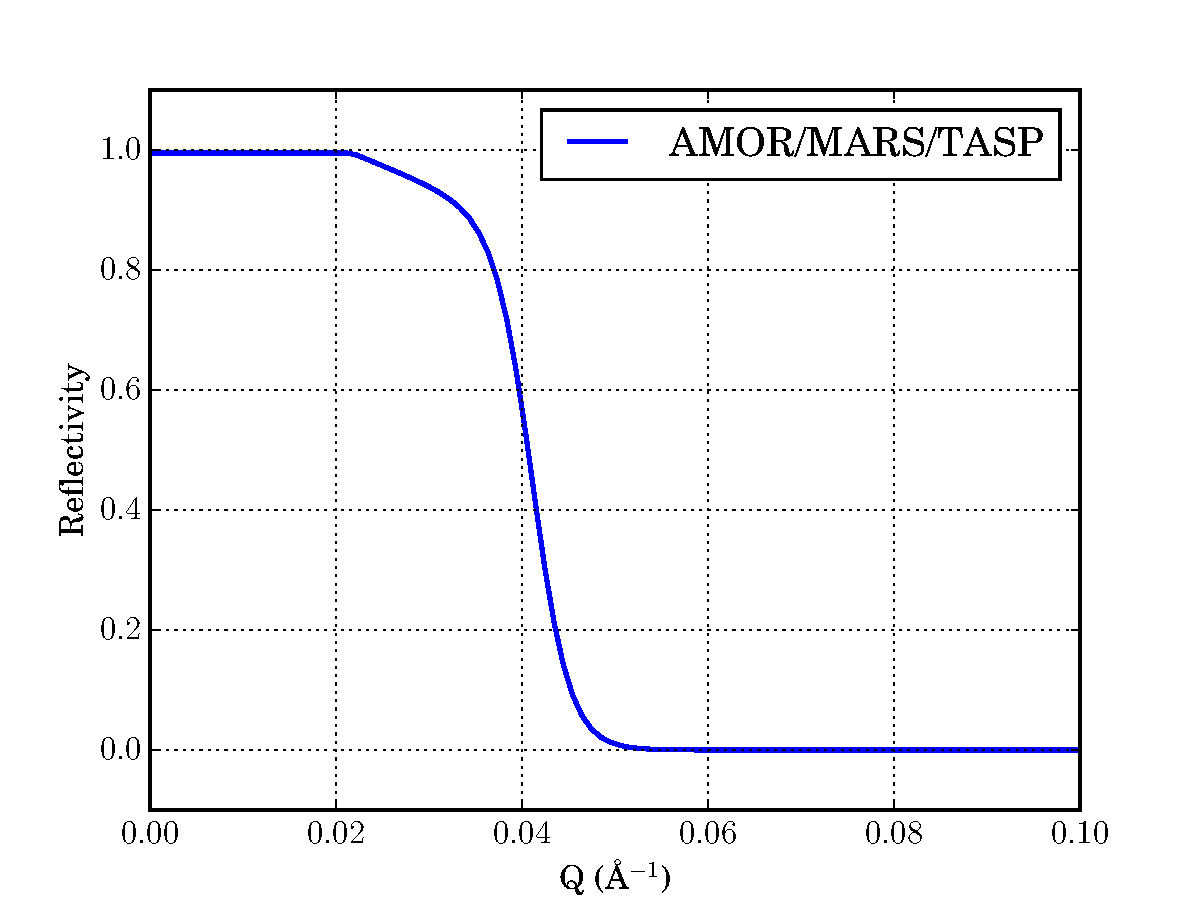
\includegraphics[scale=.4]{graphics/refl.pdf}
\caption{\label{SINQ_reflectivity} The reflectivity curve of the current SINQ neutron guides.}
\end{minipage}\hspace{5pc}%
\begin{minipage}{11pc}
\begin{multline}\label{eq:ref}\scriptsize
R(Q) = 
\begin{cases}
    \mbox{if } Q > Q_c : \\
    \frac{R_0}{2}\left\{  1 - \tanh\left(  \frac{Q - m Q_c}{W}\right) \right\}\{1-\alpha(Q-Q_c)\} \\
    \\
    \mbox{if } Q \leq Q_c :\\
    R_0 \\
\end{cases} \\ \\ \\
\begin{tabular}{c c c}
$R_0=0.995$ & $Q_c=2.17\times10^{-2}\AA^{-1}$ & $m=1.9$ \\ 
$\alpha=6.40 \AA$ & $W=4.0\times10^{-3} \AA^{-1}$ 
\end{tabular} \\
\end{multline}
\end{minipage} 
\end{figure}

Since the neutron reflection probability is based on momentum transfer and the reflections are specular, the probability is determined by the incident neutron angle and energy.  If the guide is rectangular, the reflection probability will not change as the neutron travels down the guide since the reflection angle remains constant.  These conditions mean that the exiting neutron current should be completely defined by the incident polar angle and energy of a neutron entering the guide.  The position in the guide entrance will determine the phase of the exiting rays, but if the entire exit surface is summed over, this phase becomes irrelevant.

\subsection{Reconstruction}

In order to approximate the neutron current exiting the guide, a number of fixed-source runs of MCNPX were done as precalculations to the parametric study.  An evenly-distributed source was defined at the entrance surface of the guide that emits neutrons in a polar angle bin $1/8^\circ$ wide and logarithmically in energy (to ensure low energies are sampled well).  The exiting current at the end of the guide was tallied and divided by the entrance current to yield a transfer function in energy for the polar angle of the source.  This was done for 0 to 7.5 degrees of polar angle to yield the set of 60 functions shown in figure \ref{xfer_func}.  Blue curves are those for incident angles that have an integer value of 0 degrees (e.g. 0.125, 0.250, etc.), green curves for 1, red curves for 2, and so on.  The set clearly shows that incident angles above 2 degrees make no contributions to wavelengths shorter than 8 \AA{} in the exit spectrum, and incident angles above 4 degrees make no contributions to wavelengths shorter than 16 \AA{}. 

%trim <left> <lower> <right> <upper>
\begin{figure}
\begin{center}
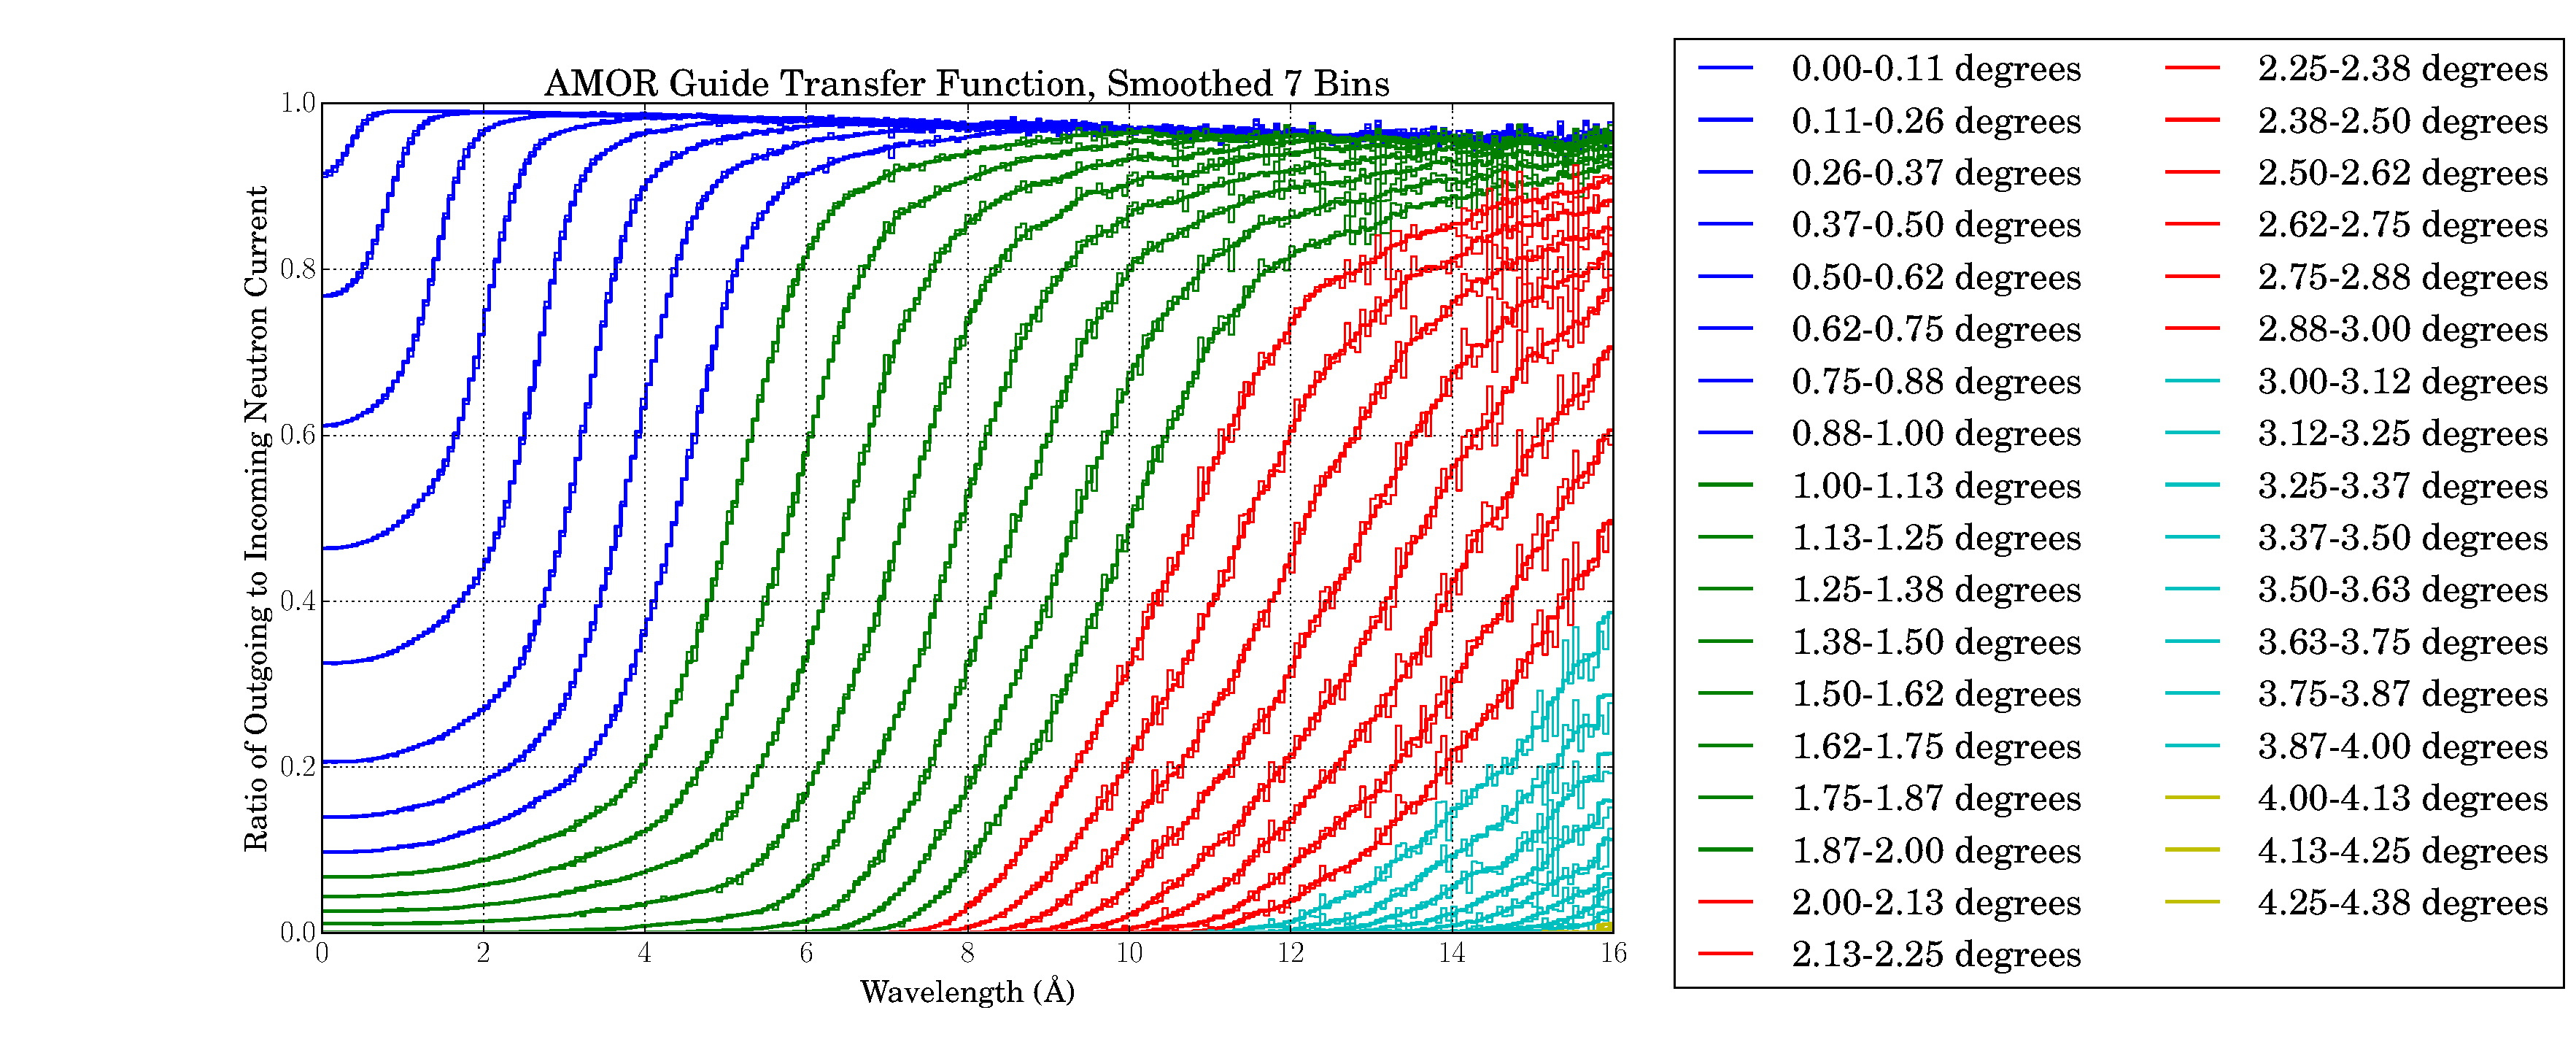
\includegraphics[scale=0.3,trim={2cm 1.7cm 1.8cm 0.8cm},clip]{graphics/xfer_func.pdf}
\end{center}
\caption{\label{xfer_func}Set of transfer functions for a m=2 guide.}
\end{figure}

If neutrons are tallied at the guide entrance in the same polar and energy binning as the transfer functions, it can be multiplied by the set and summed over all incident angles to yield the integrated neutron spectrum at the guide exit.  This way, the reflectivity model can be eliminated from the transport runs and a good estimate of the exiting current can still be made.

\subsection{Self-Consistency Test}

In order to verify that the reconstruction method works as expected, a comparison was made to an exit spectrum calculated with reflectivity model activated.  As mentioned previously, a surface source was first written at the guide entrance, then this was used as the source for a second run with the guide reflectivity model activated.  During the second run, the entry and exit current was tallied.  The entry current was binned in polar angle according to the divisions in the pre-calculated transfer functions.  The exit spectrum was the approximated by   The results of the comparison are shown in Figure \ref{xfer_bench}.  The green line is the total, integrated neutron spectrum at the guide entrance, the blue line is the integrated exit current that was trnaported by the reflectivity model and tallied at the guide exit (the benchmark), and the red curve is the reconstructed exit spectrum.  The maximum error seen is about 70\% at 0.55 \AA{}, but decreases with energy and is almost always within the statistical error of the simulation.  The average 1-norm value (norm divided by number of bins) of the relative error is 7.8\%, and the average 2-norm value is 0.8\%.

\begin{figure}
\begin{center}
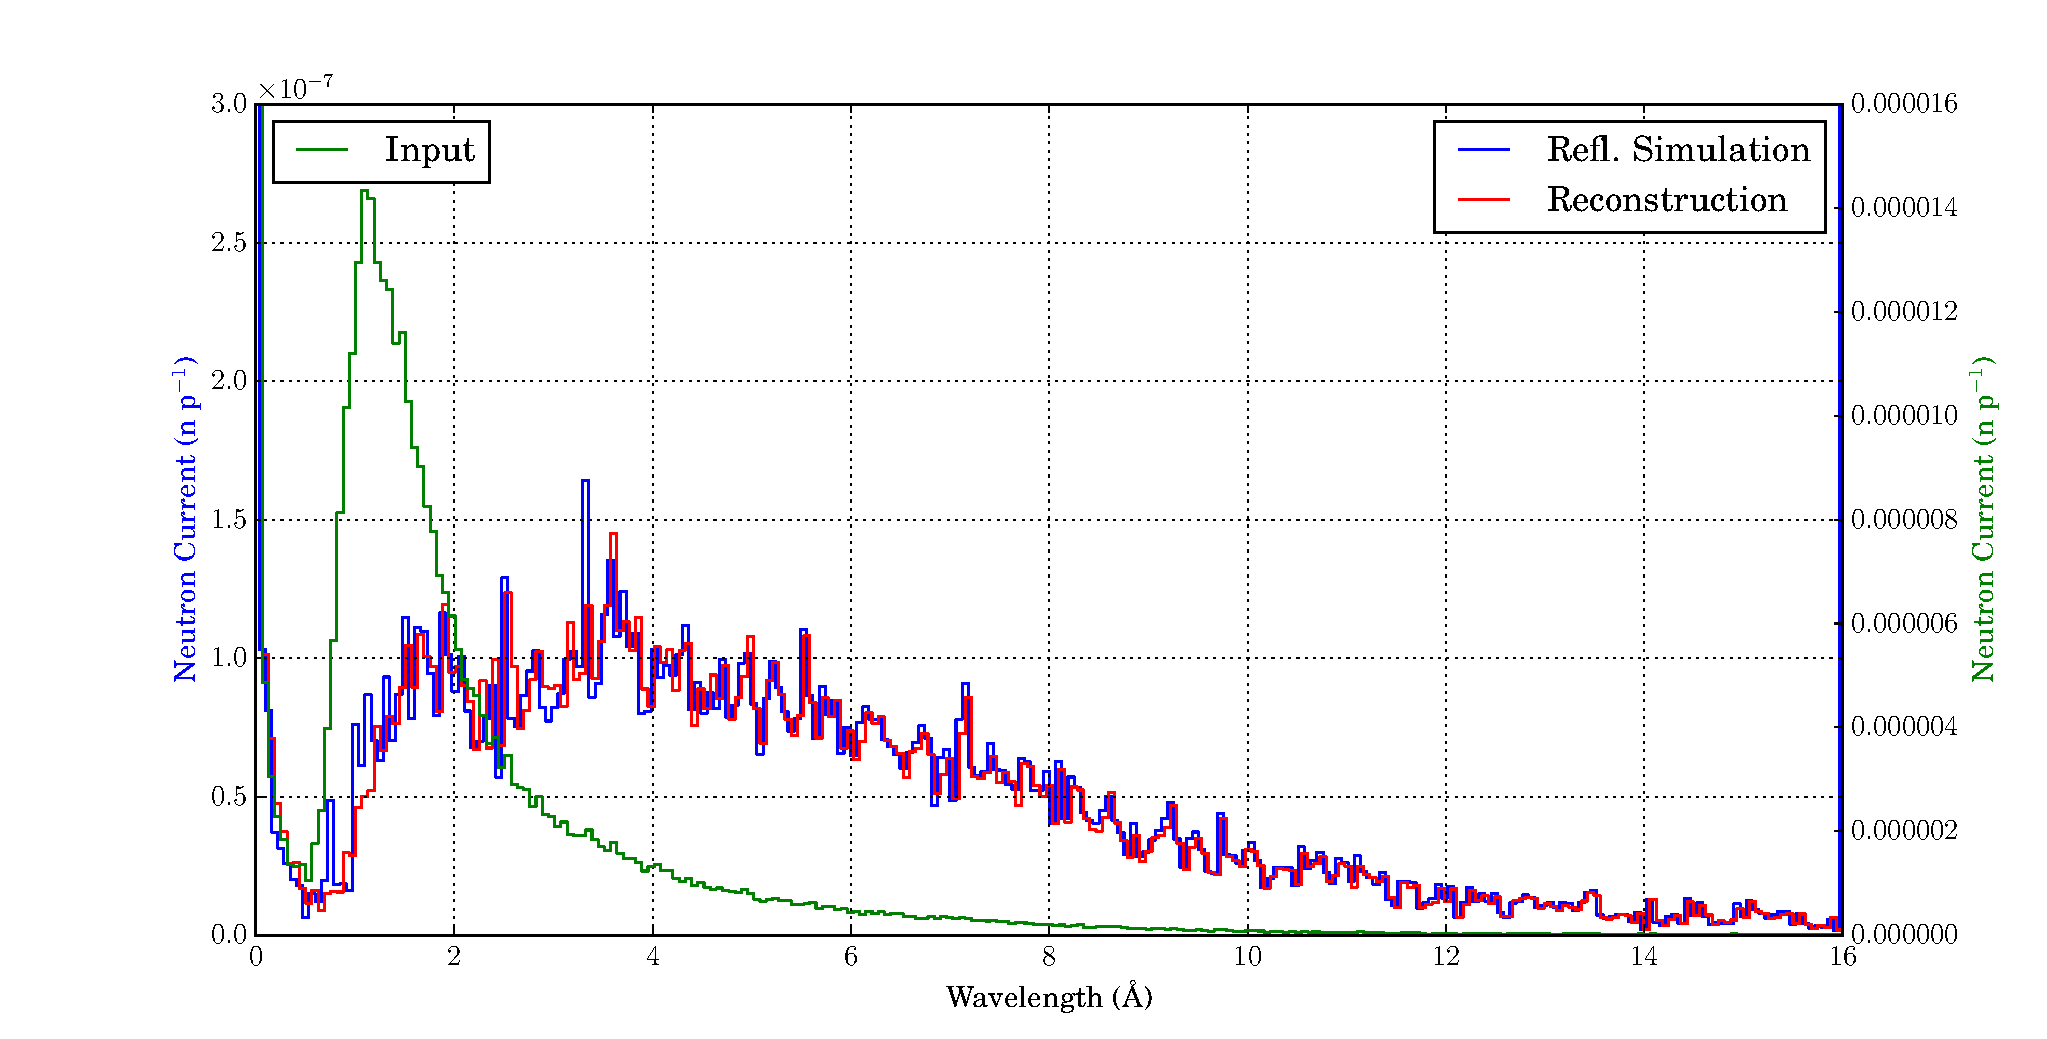
\includegraphics[scale=0.5]{graphics/xfer_bench.pdf}
\end{center}
\caption{\label{xfer_bench}The reconstructed guide exit current compared to the exit current calculated with a MCNP simulation with guide reflectivity activated.  The right axis is for the exit spectra and the left axis is for the entrance spectrum.  The lower plot shows the recontruction relative error compared to the reflectivity simulation.  The green envelope is the 1-sigma relative error of the reflectivity simulation.}
\end{figure}

\section{REH Parametric Study in the Horizontal Plane}

The re-entrant hole parametric study was done to investigate a wide range of geometries in the horizontal plane, where the guide width is smaller than the hole size and all the guides have different view angles.  Four REH depths (14, 10, 6, 2 cm), four opening widths (4, 8, 12, 16 cm), and eleven hole slopes (-0.5, -0.4, -0.3, -0.2, -0.1, 0.0, 0.1, 0.2, 0.3, 0.4, 0.5) were investigated in the study, totalling 176 cases. Figure \ref{parametric_geom} shows the parameters in relation to the cold source geometry.  The REH vertical dimensions were chosen to be the full width of the nozzle with a slightly tapering inward slope.  The vertical dimensions were kept constant in this study, but will be the focus of future work.

\begin{figure}[h]
\begin{minipage}{14pc}
\begin{center}
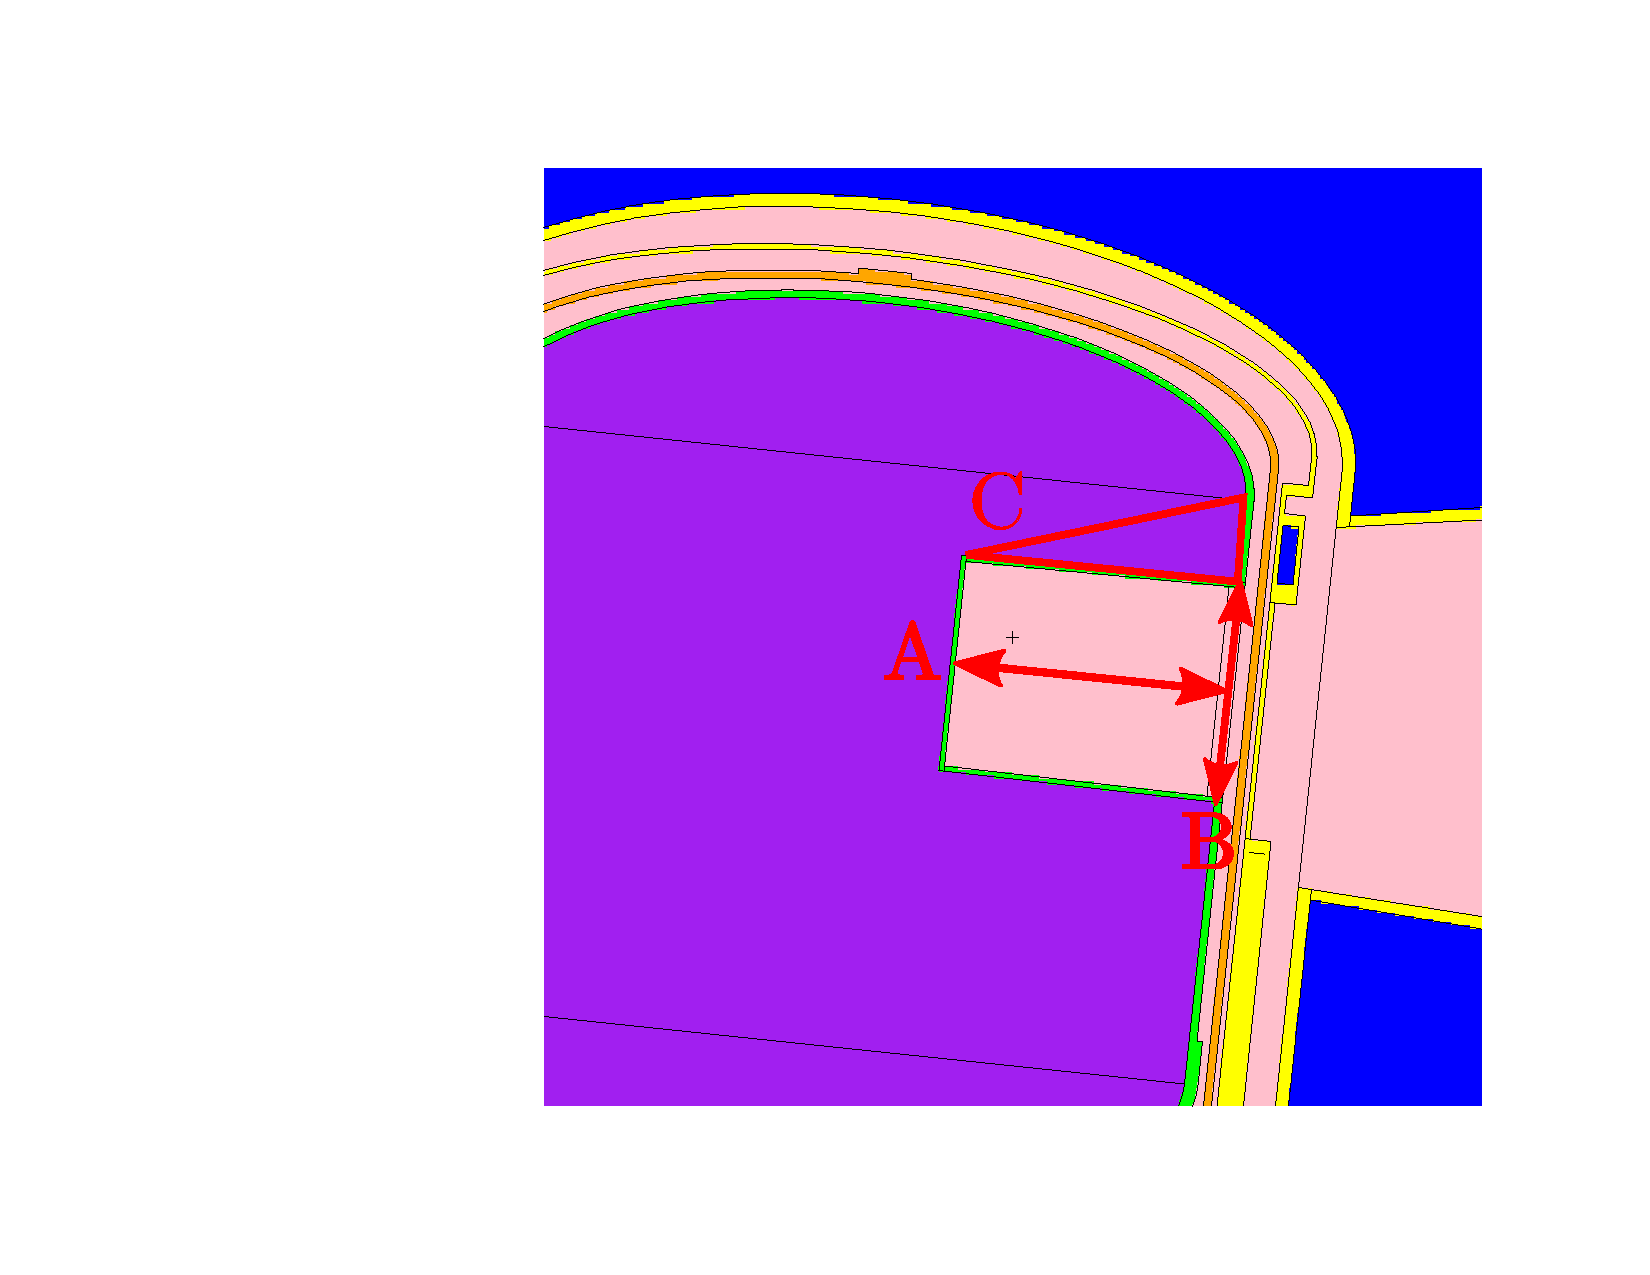
\includegraphics[scale=0.4,trim={13cm 6cm 4cm 5cm},clip]{graphics/para_geom.pdf}
\end{center}
\caption{\label{parametric_geom}The geometry varied in the REH parametric study. ``A'' is the hole depth, ``B'' is the opening width, and ``C'' is the hole slope.}
\end{minipage}\hfill%
\begin{minipage}{11pc}
\begin{center}
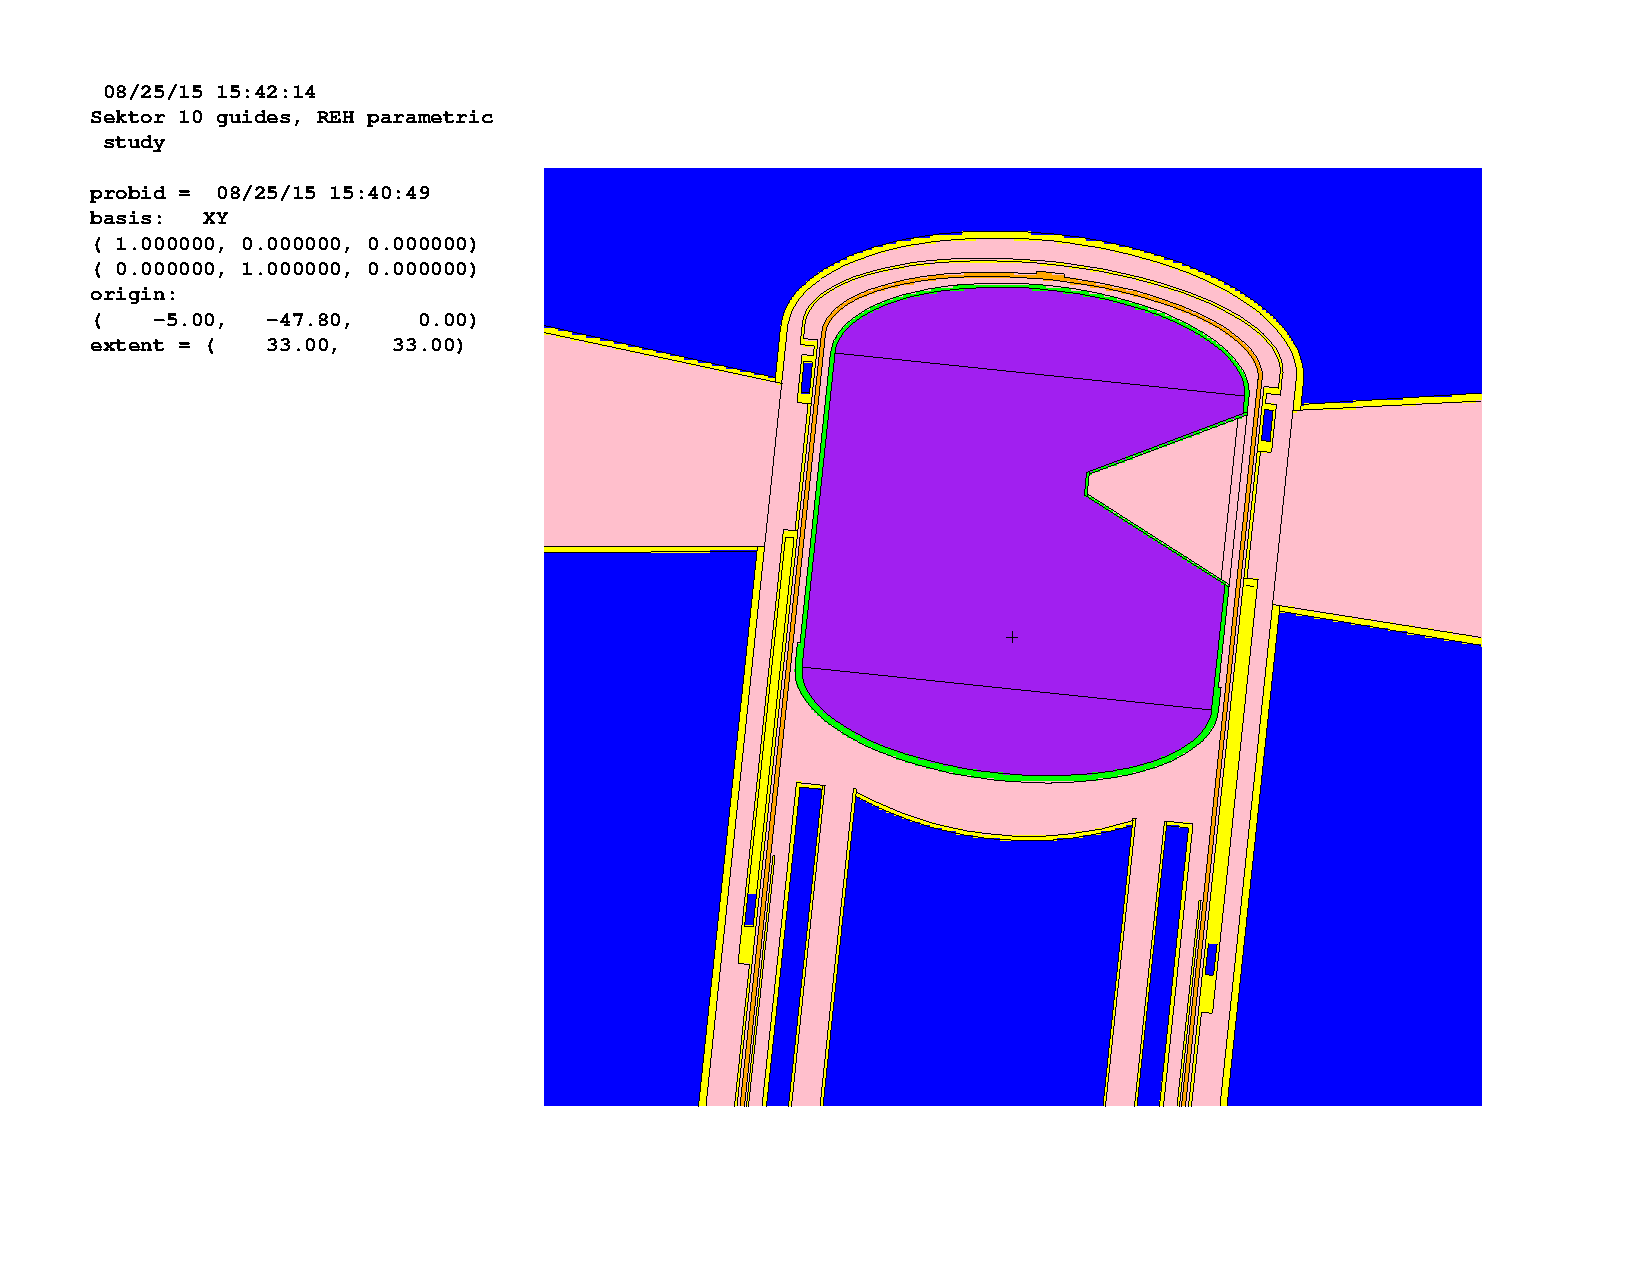
\includegraphics[scale=0.4,trim={11.2cm 8cm 5cm 3cm},clip]{graphics/case077.pdf}
\end{center}
\caption{\label{case077}The best-performing horizontal geometry for the REH.}
\end{minipage} 
\end{figure}

With all of the variance reduction and approximations implemented, each case took about one hour to run on a 144-core configuration on a computer cluster at PSI.  The spectra from all the cases are shown in upper plot of Figure \ref{parametric_REH}, and their figures of merit are shown in the lower plot.  The figure of merit was chosen to be the total current exiting the guide from 3 to 6 \AA{} -- the wavelength band which is useful for most of the instruments in the guide hall \cite{intruments_wavelength}.  The parameters were varied in slope-width-depth order, with slope being the fasted varied parameter. Figure \ref{parametric_REH} has labeled, colored blocks in the lower plot to show which parameters are constant for that block.  Slope and opening width have the most affect on exit current at large hole depths.

The geometry of the best-performing case is shown in figure \ref{case077}.  The depth is 10 cm, the opening width is 12 cm, and the slope is 0.5.  This opening is as wide as the nozzle and almost tapers to a point at the maximum depth.  The maximum depth is 4 cm from the radial center of the cold source.  

\begin{figure}
\begin{center}
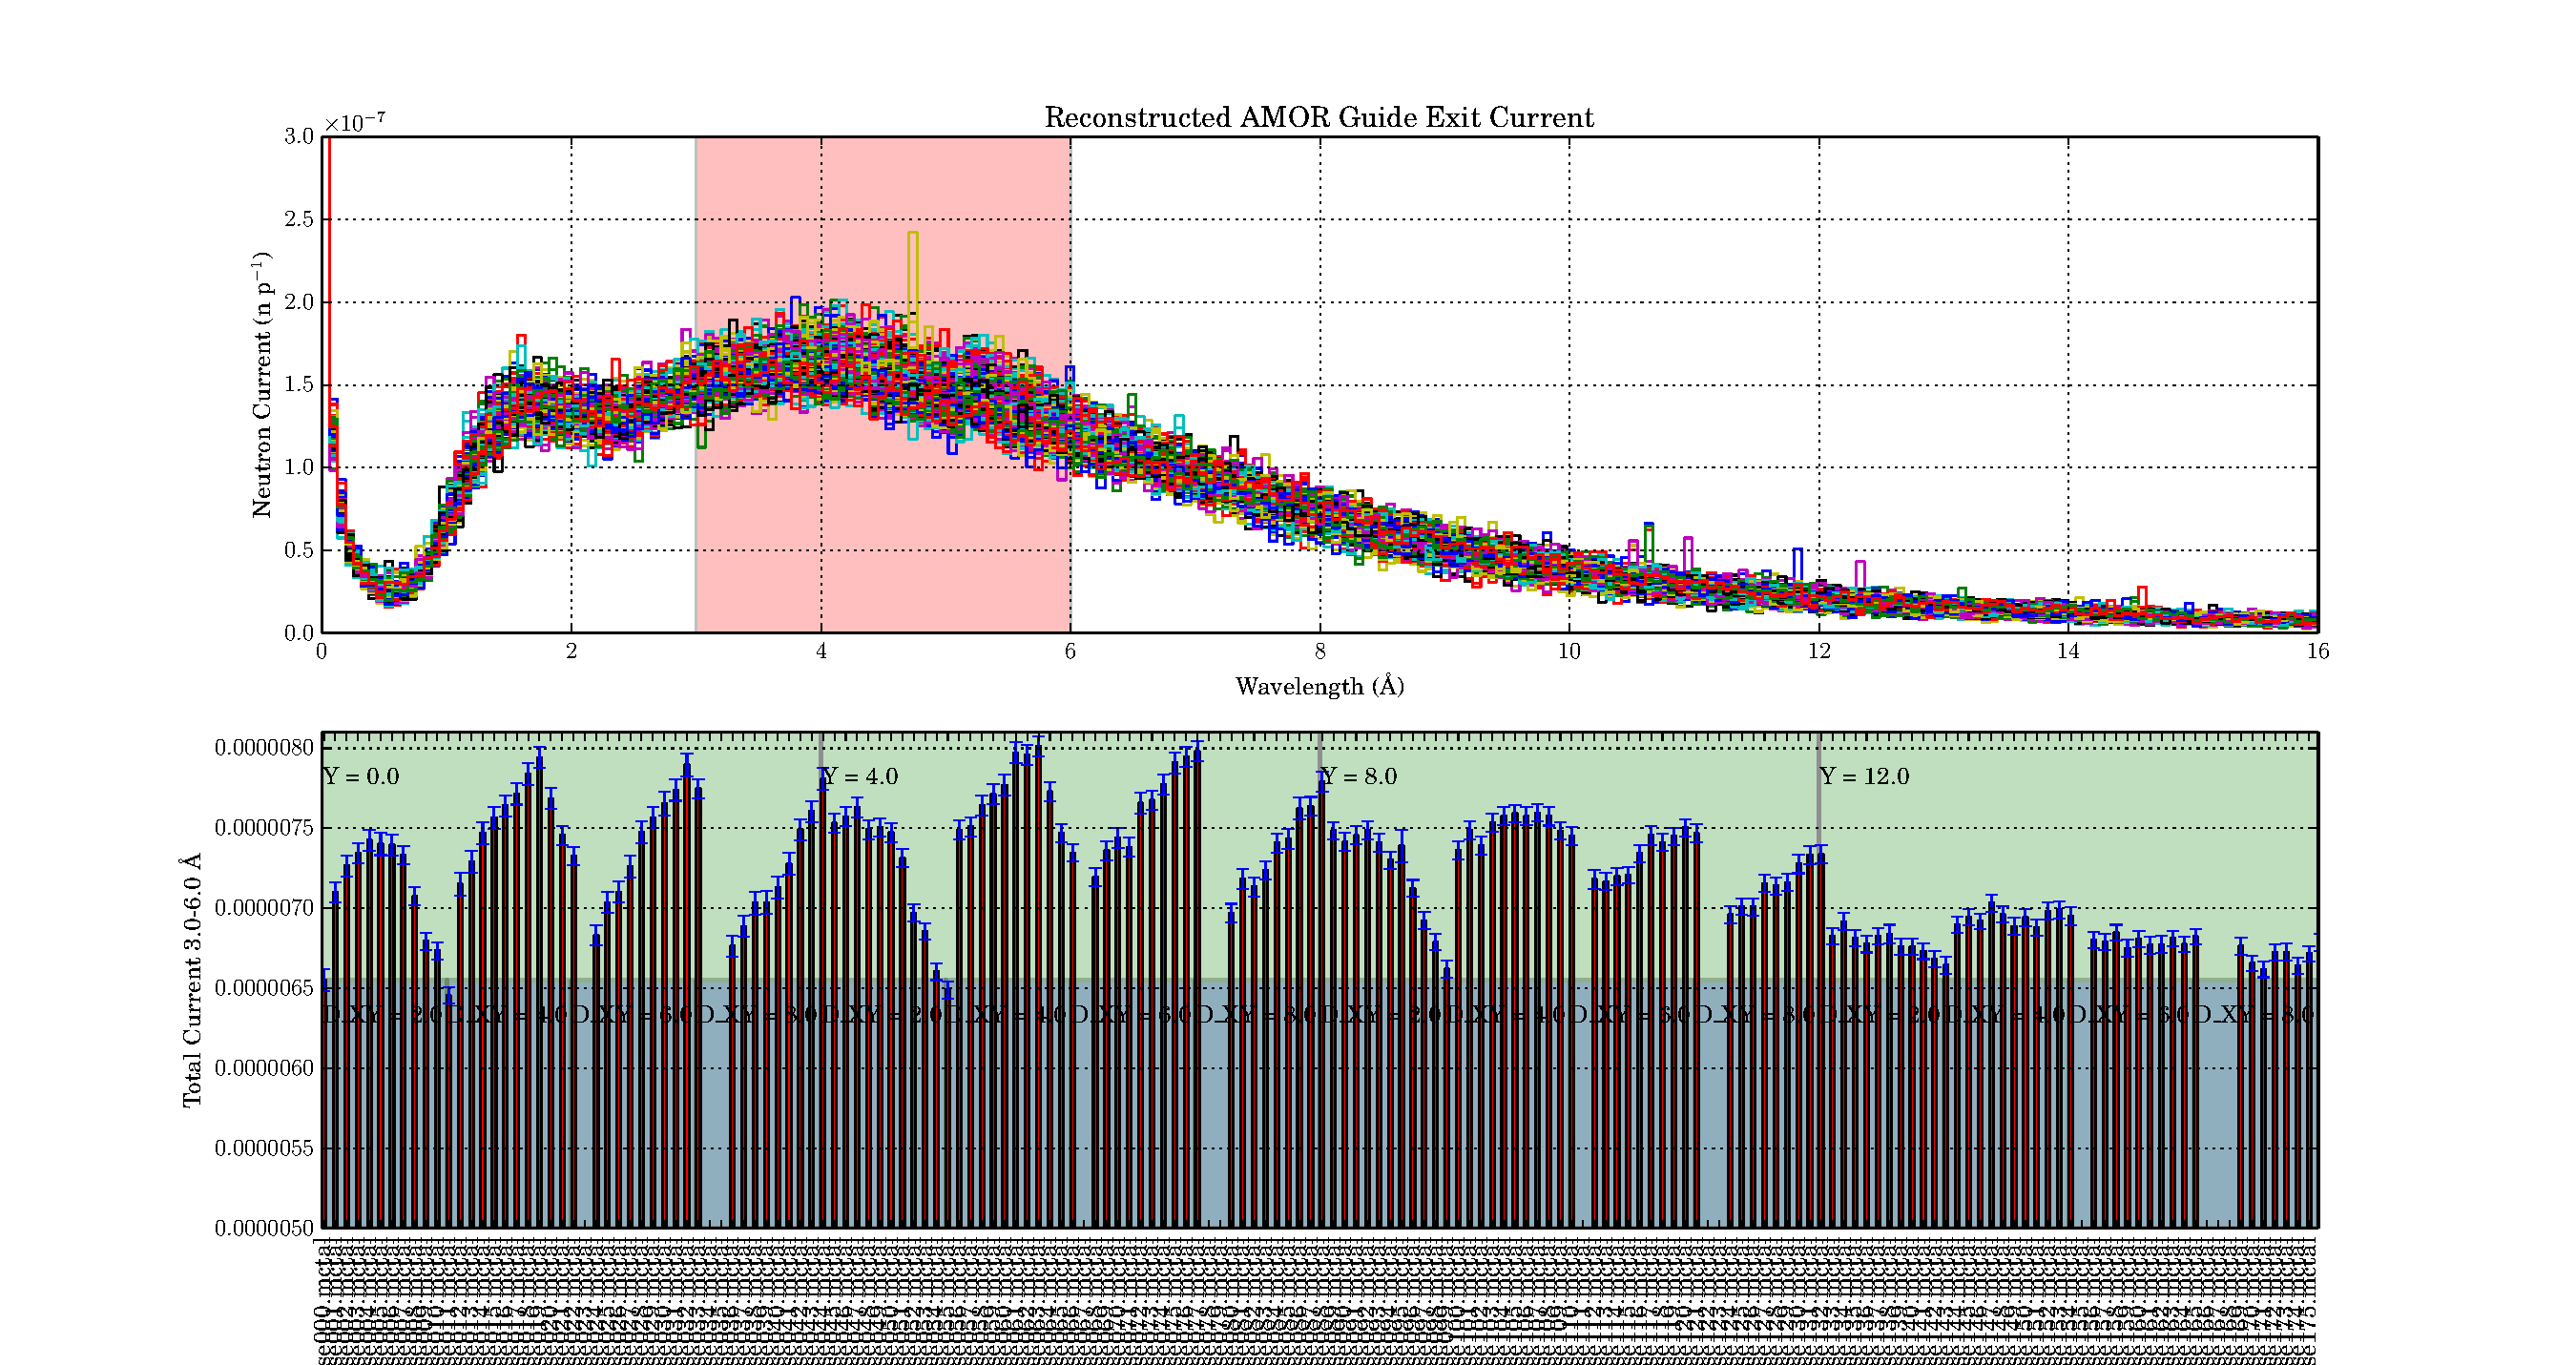
\includegraphics[scale=0.38,trim={1cm 2.35cm 1cm 0cm},clip]{graphics/parametric_REH.pdf}
\end{center}
\caption{\label{parametric_REH}The envelope formed by the spectra from all 176 cases considered (upper) and their figures of merit (lower) which is total current from 3 to 6 \AA{}.}
\end{figure}

\begin{figure}
\begin{center}
\includegraphics[scale=0.38,trim={0cm 0cm 0cm 0cm},clip]{graphics/parametric_gain.pdf}
\end{center}
\caption{\label{parametric_gain}The gain factor of the neutron guide exit current of best-performing REH geometry over the REH being absent.  The thick red line is the data smoothed over 15 bins.}
\end{figure}


Figure \ref{parametric_gain} shows the gain from the best performing REH geometry over an absent REH.  The maximum gain 1.29 at 5.5 \AA{} and its average value from 3-6 \AA{} is 1.24.  Similar gains should be seen by all instruments in the SINQ guide hall.  The drop in gain after 5.5 \AA{} is suspected to be from the liquid D$_2$ cross section dropping from about 5.5 to 25 \AA{}, making it more transparent to colder neutrons and reducing the re-entrant hole's benefits.


\section{Conculsions}

From this study, it can be concluded that the flux reconstruction method is at least self-consistent, and that a near-optimal horizontal REH geometry has been determined.  The REH increases total exit current by a factor of 1.24 on average from 3-6 \AA{} with a peak gain of 1.29 at 5.5 \AA{}.

\section{Future Work}

This study has only determined the horizontal geometry of the re-entrant hole in the cold source at SINQ.  Another study is needed to investigate REH sensitivity to vertical changes, as well as a parametric study over a smaller range near the optimal point to determine more exact dimensions.  The affect the REH has on the neutron flux on the opposite side will also be determined.

Different types of reflector materials and configurations will also be investigated.  The refector sits behind the cold source (the side opposite the target), and reducing cold neutron losses in it may increase the guide exit current.  Adding a belt of liquid H$_2$ to produce a ``cold spot'' for focusing instruments will also be investigated.  In these studies, the flux reconstruction method will once again be used.

A guide reflectivity patch will be made for MCNP 6.1 will also be done.  Ideally, it will also include a switch to reduce neutron weight upon reflection instead of leaking non-reflected neutrons. This should help speed up in-beam calculations where this signal is of interest and not the noise.

\section*{References}
\bibliography{paper}


\end{document}
